\documentclass[11pt]{article}
\usepackage[includeheadfoot, top=1.0in, bottom=1.0in, hmargin=1.0in]{geometry}
\usepackage[utf8]{inputenc}
\usepackage{fancyhdr}
\usepackage{url}
\pagestyle{fancy}
\usepackage{setspace}
\usepackage{tabularx}
\usepackage{graphicx}
\usepackage{caption}
\usepackage{subcaption}
\usepackage{hyperref}
\usepackage{multicol}

\usepackage{hyperref}
\hypersetup{
    colorlinks=true,
    linkcolor=blue,
    filecolor=magenta,      
    urlcolor=blue,
}


\lhead{Astronomy Lab II}
\rhead{Spring 2022}
\lfoot{Mead}
\rfoot{Mon 6-9pm}
\cfoot{\thepage}

\begin{document}

\begin{center}
\huge{Lab 4: Galaxy Classification}\\ \medskip \Large{February 14, 2022}
\end{center}

%%%%%%%%%%%%%%%%%%%%%%% INTRO %%%%%%%%%%%%%%%%%%%%%%%
\section{Introduction: In a Galaxy Far, Far Away}
In the early 20$^{th}$ century, there was a deep tension in astronomy about the nature of some faint, fuzzy objects astronomers could barely make out with their telescopes. Some astronomers believed these ``nebulae" were clusters of stars in our own Galaxy, while others believed that they were actually great, distant islands of stars much like our own Milky Way.  This was known as \textit{The Great Debate}.  It wasn't until 1924 when Edwin Hubble measured the distance to one of these ``nebulae" that astronomers were able to settle this debate. Hubble measured the distance to the Andromeda Galaxy to be over 2 million light years away, confirming it was indeed a galaxy far, far away (cue \href{https://www.youtube.com/watch?v=MNMSAIG0dfQ}{Star Wars music}), and that our Universe is more vast than we can possibly imagine.

\medskip \noindent
Since Hubble's discovery, astronomers have studied galaxies with great interest. Galaxies come in all shapes, sizes, colors, and luminosities.  Each of these properties can tell us something unique about galaxies -- from what stage of their evolution they are in, to something about the stars that live in them, to where the galaxies themselves live, to how much of the mysterious dark matter they have.  The first step in understanding how galaxies work is to know what kind of galaxy you have, just by looking at it!  Today, we will think about the \textit{morphology}, or shape, of galaxies and what we can learn from that.  The goals of today's lab are for you to get a sense of the diversity of galaxies, create and test a classification system of your own, and learn about what the morphology of a galaxy can tell us about its evolutionary state.

%%%%%%%%%%%%%%%%%%%%%%% MAKE YOUR OWN CLASSIFICATION %%%%%%%%%%%%%%%%%%%%%%%
\section{Classifying Galaxies}
\subsection{Make Your Own Classification System}

\begin{enumerate}
    \item Break up into groups of 2-3.  With your group, navigate to \url{http://cas.sdss.org/dr7/en/proj/advanced/galaxies/} and click ``Next".  You should see a table with 3 columns, recording information about an image.  In the ``Field" column, you should be able to click on a link in each row that will take you to an image of one or more galaxies.  Look through the images and spend a little time thinking about what is similar or different about each galaxy.  What characteristics stand out?
    \item Come up with a method of classifying the galaxies.  You can do this by any means you like, although remember that all the images are at different distances and thus the perceived brightness and size will be different than the actual brightness or size.
    \item In your lab book, write out a series of steps or a visual representation of how your method works.  Make sure it is clear enough that someone else can use it.
    \item Once you've finished writing, find the Hercules Cluster image under Files on Courseworks.  Using your method, classify each labeled galaxy.  How robust is your system?  Comment, in your lab notebook, on what, if any, faults your method may have.  Would it still be useful for images in X-ray or radio?  Thinking a little about our previous lab `The Multiwavelength Universe' will help you answer this question.
    \item Now we will get together as a class, discuss the different classification systems you came up with, and come to a consensus for how to classify galaxies.
\end{enumerate}

%%%%%%%%%%%%%%%%%%%%%%% GALAXY ZOO %%%%%%%%%%%%%%%%%%%%%%%
\subsection{Galaxy Zoo}

Navigate to \url{https://www.zooniverse.org/projects/zookeeper/galaxy-zoo/}.  Galaxy Zoo is a citizen science project that leverages the number of people with even just a casual interest in astronomy to categorize large data sets of galaxy images.  Once you are on the Galaxy Zoo main page, click ``Get Started".  Read through the instructions, but if you ever need help with the task, you can click on ``Need some help with this task?" or the ``Field Guide" off to the right.  I highly recommend looking through some of the examples under ``Need some help with this task?" for each of the questions for the first galaxy you look at.

\medskip \noindent
Spend about 10-15 minutes classifying galaxies on Galaxy Zoo and do the following for each galaxy that you see.
\begin{enumerate}
    \item In a table in your lab notebook, keep a tally of how many galaxies of each type you see using the classification system we came up with in class.
    \item Answer the questions that you are asked in Galaxy Zoo.
\end{enumerate}
Once 10-15 minutes are up, in your lab notebook, \textbf{briefly reflect on anything unusual you saw and how it might make using the classification system we came up with as a class difficult. How could we improve our class classification system?}

%%%%%%%%%%%%%%%%%%%%%%% HUBBLE TUNING FORK %%%%%%%%%%%%%%%%%%%%%%%
\section{Cue the Music - The Hubble Tuning Fork}

\begin{figure} [h!]
    \centering
    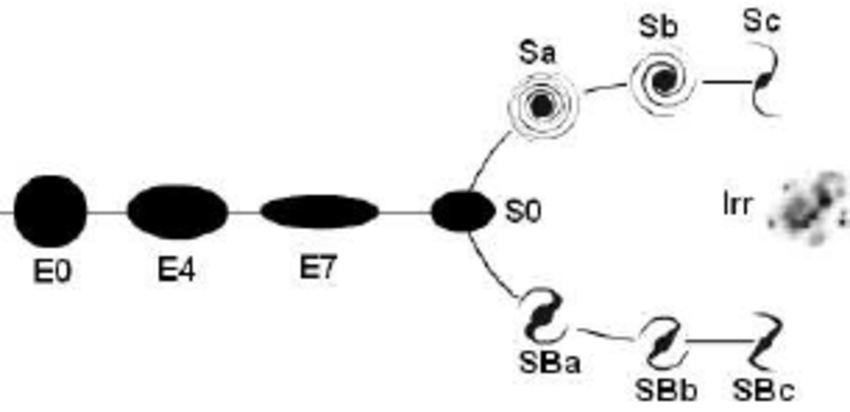
\includegraphics[width=0.7\textwidth]{Images/The-Hubble-tuning-fork.png}
    \caption{The Hubble Tuning Fork}
    \label{fig:Hubble}
\end{figure}

\noindent
Figure \ref{fig:Hubble} is a schematic of the galaxy classification system that astronomers use -- it is known as the \textit{Hubble Tuning Fork}. The Hubble sequence is a morphological classification scheme for galaxies invented by Edwin Hubble in 1936. It is known colloquially as the Hubble Tuning Fork because of the shape in which it is traditionally represented. Hubble's scheme divides galaxies into 3 broad classes based on their visual appearance. \textbf{Answer the following in your lab notebook}:

\begin{enumerate}
    \item There are 3 branches on the tuning fork.  Describe what features you think each branch is representing, and how the galaxies along each branch differ.
    \item How does the Hubble Tuning Fork compare with the galaxy classification system we came up with in class?
\end{enumerate}

\pagebreak
\noindent
You probably noted some of the following features in your description of the Hubble Tuning Fork.  Here are the formal names and descriptions for the galaxy types represented in Hubble's classification system.

\begin{enumerate}
    \item \underline{Elliptical galaxies} have smooth, featureless light distributions and appear as ellipses in images. They are denoted by the letter E, followed by an integer n representing their degree of ellipticity (how close to circular they are) on the sky.
    \item \underline{Spiral galaxies} consist of a flattened disk, with stars forming a (usually two-armed) spiral structure, and a central concentration of stars known as the bulge, which is similar in appearance to an elliptical galaxy. They are given the symbol S. Roughly half of all spirals are also observed to have a bar-like structure, extending from the central bulge. These barred spirals are given the symbol SB.
    \item \underline{Lenticular galaxies} (designated S0) also consist of a bright central bulge surrounded by an extended, disk-like structure but, unlike spiral galaxies, the disks of lenticular galaxies have no visible spiral structure and are not actively forming stars in any significant quantity.
    \item \underline{Irregular Galaxies} do not fit into the Hubble sequence, because they have no regular structure (either disk-like or ellipsoidal). 
\end{enumerate}


\noindent
\textbf{Here's a fun fact:} The Hubble Tuning Fork is drawn the way it is because astronomers originally thought galaxy morphologies evolved from left to right.  They thought galaxies were formed as \textit{elliptical} galaxies, then evolved into \textit{spiral} galaxies, and finally morphed into \textit{irregular} galaxies.  We now think that galaxies do the exact opposite, and are born as irregular galaxies, form spirals through interactions with other galaxies, and finally end up as elliptical, featureless galaxies.

\pagebreak
\subsection{The Hubble Ultra Deep Field}
%Introduce the Hubble Deep Field

Navigate to \url{https://cdn.spacetelescope.org/archives/images/large/heic0406a.jpg}.
\\\textbf{\textit{Whoa}}, right? This image is known as the \textit{Hubble Ultra Deep Field}. The snapshot includes galaxies of various ages, sizes, shapes, and colors. The smallest, reddest galaxies may be among the most distant known, existing when the universe was just 800 million years old. The nearest galaxies - the larger, brighter, well-defined spirals and ellipticals - thrived about 1 billion years ago, when the cosmos was 13 billion years old.

\medskip \noindent
The image required 800 exposures taken over the course of 400 orbits of the Hubble Telescope around Earth. The total amount of exposure time was 11.3 days, taken between Sept. 24, 2003 and Jan. 16, 2004.

\medskip \noindent
\textbf{Do the following in your lab notebooks:}
\begin{enumerate}
    \item With the exception of a few stars in this image, every object you see is a galaxy.  Try to identify the stars. How did you identify them?
    \item Estimate the number of galaxies you see in the Hubble Ultra Deep Field.
    \item Does these seem reasonable, weird, outrageous?  About what fraction are spiral galaxies?  What fraction are elliptical galaxies?
    \item Why are some galaxies larger than others?
\end{enumerate}


%%%%%%%%%%%%%%%%%%%%%%% OBSERVING %%%%%%%%%%%%%%%%%%%%%%%
\section{Observing}
Now, we will go look at our very own set of galaxies using the telescope.  \textbf{In a table in your lab notebook, take down some observations for each galaxy we look at.}  You may want to consider the galaxy's morphology (use the Hubble Tuning Fork), whether or not it is facing us or if it is edge-on, any unique or distinct features, etc.  If you are finding it difficult to classify the galaxies, \textbf{why}?

%%%%%%%%%%%%%%%%%%%%%%% CONCLUSIONS %%%%%%%%%%%%%%%%%%%%%%%
\section{Conclusions}

\begin{enumerate}
    \item Considering the wide variety of galaxies that you saw in the Hubble Ultra Deep Field image, what are some other features of galaxies we could account for, besides morphology?
    \item What might make classifying a galaxy difficult?
    \item Do you have any feedback about this lab?
    \item There is nothing to complete for this item, however, there are many citizen science research projects like the Galaxy Zoo that YOU can participate in. Check some of them out here: \url{https://www.zooniverse.org/projects?discipline=astronomy&page=1&status=live}
\end{enumerate}


\end{document}
